\documentclass[a4paper, 12pt]{article} % Размер бумаги устанавливаем А4, шрифт 12 пунктов

\usepackage{cmap} % Поиск по русским символам в полученном PDF
%\usepackage{mathpazo} % Шрифт

\usepackage[T1,T2A]{fontenc} % Использовать смешанный язык в PDF документе
\linespread{1.05} % Межстрочное расстояние
\usepackage[utf8]{inputenc} % lex файл использует кодировку utf8
\usepackage[english,russian]{babel} % Используем русский и английский языки с переносами

\usepackage{amsmath} % Математические символы
\usepackage{url} % Позволяет вставлять ссылки

\usepackage{graphicx} % Позволяет вставлять картинки
\usepackage{wrapfig} % Обтекание картинок текстом

\DeclareUnicodeCharacter{00A0}{~} % Решение проблемы затупов LaTeX

\usepackage{listings} % Листинг
\usepackage{xcolor} % Цвета в тексте
\definecolor{sh_comment}{rgb}{0.12, 0.38, 0.18 } %adjusted, in Eclipse: {0.25, 0.42, 0.30 } = #3F6A4D
\definecolor{sh_keyword}{rgb}{0.37, 0.08, 0.25}  % #5F1441
\definecolor{sh_string}{rgb}{0.06, 0.10, 0.98} % #101AF9
% Подсветка кода в стиле eclipse
\lstset{
    frame=tb, % draw a frame at the top and bottom of the code block
    tabsize=4, % tab space width
    basicstyle=\small,
    showstringspaces=false, % don't mark spaces in strings
    numbers=left, % display line numbers on the left
    stringstyle=\color{sh_string},
    keywordstyle = \color{sh_keyword}\bfseries,
    commentstyle=\color{sh_comment}\itshape % string color
}

\makeatletter
\renewcommand\@biblabel[1]{\textbf{#1.}} % Change the square brackets for each bibliography item from '[1]' to '1.'
\renewcommand{\@listI}{\itemsep=0pt} % Reduce the space between items in the itemize and enumerate environments and the bibliography

\renewcommand{\maketitle}{ % Customize the title - do not edit title and author name here, see the TITLE block below
\begin{flushright} % Right align
{\LARGE\@title} % Increase the font size of the title

\vspace{50pt} % Some vertical space between the title and author name

{\large\@author} % Author name
\\\@date % Date

\vspace{40pt} % Some vertical space between the author block and abstract
\end{flushright}
}

\setlength{\parskip}{\baselineskip} % Вертикальный отступ между абзацами
\setlength\parindent{0pt} % без красных строк

%----------------------------------------------------------------------------------------
%	TITLE
%----------------------------------------------------------------------------------------

\title{\textbf{Системное программирование}\\ % Title
Современные проблемы} % Subtitle

\author{\textsc{Мартынов Семён} % Author
\\{\textit{Санкт-Петербургский государственный\\ Политехнический университет}}} % Institution

\date{\today} % Date

%----------------------------------------------------------------------------------------

\begin{document}

\maketitle % Print the title section

%----------------------------------------------------------------------------------------
%	ABSTRACT AND KEYWORDS
%----------------------------------------------------------------------------------------

%\renewcommand{\abstractname}{Summary} % Uncomment to change the name of the abstract to something else

\begin{abstract}

В системном программировании существуют два вектора развития - обеспечение работы с аппаратурой и предоставление определённых условий работы прикладному ПО. Я рассмотрю те сложности, которые возникли перед системными программистами за последние 7 - 10 лет. Некоторые из этих проблем актуальны и для программистов прикладных, но данной работе акцент сделан именно на разработке системного ПО.
\end{abstract}

\hspace*{3,6mm}\textit{Ключевые слова:} системное программирование, сложность, параллельное исполнение, верификация % Keywords

\vspace{30pt} % Some vertical space between the abstract and first section

%----------------------------------------------------------------------------------------
%	ESSAY BODY
%----------------------------------------------------------------------------------------

\section*{Введение}

Перед тем, как говорить о современных проблемах системного программирования, нужно определить, что это такое. Традиционно, системное программирование связывают с разработкой программного обеспечения (ПО), управляющего компонентами компьютерной системы. Это программное обеспечение выступает своеобразным мостом, между аппаратурой и миром прикладного ПО. Если задачами прикладных программ является решение конкретных практических задач (того, что нужно пользователю), то системное ПО должно предоставлять прикладному определённый уровень гарантий (того, что нужно программе пользователя), абстрагируя физические устройства. Со временем, объёмы и потребности прикладного ПО возросли, а вместе с тем возросли и требования к тому контексту, который обеспечиваются системным ПО. Другими словами, если раньше системное ПО было нацелено вниз, на уровень железа, операционных систем и драйверов, то сейчас системное ПО получило дополнительный вектор развития вверх, в сторону прикладного ПО, которому нужно обеспечить надёжность, переносимость и даже безопасность. Задачей системного ПО стала работа с прикладными программами как с данными, т.е. анализ, выполнение, улучшение и проверка того, что запускает пользователь. 

%------------------------------------------------

\section*{Рост сложности кода}

При традиционном рассмотрении вопроса, в первую очередь называются операционные системы. На моём ноутбуке установлена ОС Arch Linux, и ядро 3.18.3. Если запустить небольшой скрипт, который подсчитает количество строк кода (в действительности этот скрипт не различает как таковой код, заголовочные файлы или строки из справочного файла, он считает все вместе) то получится 18 998 896. Это достаточно большое число само по себе, такой объём кода невозможно держать в голове, при этом необходимо этот код поддерживать (тестировать, находить и исправлять уязвимости, обеспечивать совместимость со старыми версиями) и развивать, добавляя новый функционал. Если посмотреть примечания к выпуску, то выяснится, что по сравнению с предыдущей версией 3.17 (представленной в августе прошлого года) данная версия ядра имеет 11200 исправлений от 1300 разработчиков, а размер патча составляет 38 Мб! Изменения затронули 9307 файлов, добавлено 485719 строк кода, удалено 355945 строк, и это только за период с августа по декабрь!

\begin{figure}[h!]
\centering
\includegraphics[scale=0.4]{res/pic001}
\caption{Рост количества строк кода в ядре Linux (размер шага по оси абсцисс 1 год, по оси ординат 10 миллионов строк).}
\end{figure}

Сайт openhub.net занимается сбором статистики по популярным открытым проектам, и на рисунок 1 видно, как изменялось количество строк кода ядра с течением времени (синим цветом показаны строчки кода, серым - строки с комментариями, зелёным - строки, используемы для оформления кода). Явно наблюдается восходящий тренд, объём кода будет продолжать расти, а вместе с ним и сложность, которая ложится на плечи разработчиков.

Разработчиков тоже становится всё больше! На рисунке 2 мы видим, что количество разработчиков, вносящих свои изменения, приблизилось к 1 000 в месяц, а количество коммитов, которые они все вместе делают каждый месяц уже превысило отметку в 5 000 (см. рис 3). Важно помнить, что каждый такой коммит должен быть получен, изучен и принят (либо не принят) ментейнером, ответственным за тот или иной участок ядра.

\begin{figure}[h!]
\centering
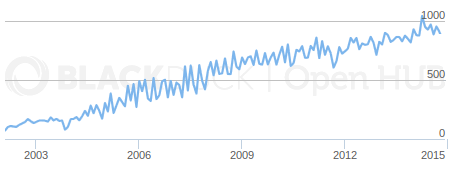
\includegraphics[scale=0.8]{res/pic002}
\caption{Рост количества разработчиков ядра Linux.}
\end{figure}

\begin{figure}[h!]
\centering
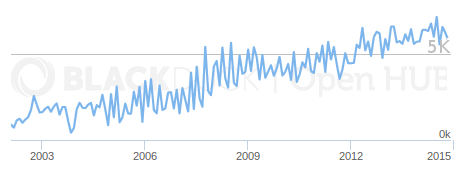
\includegraphics[scale=0.8]{res/pic003}
\caption{Рост количества изменений, предлагаемых разработчиками.}
\end{figure}

%------------------------------------------------

\section*{Экспоненциальный рост количества\\ компьютерной техники}

Помимо роста сложности кода, растёт и количество устройств, на которых этот кода работает. Объем рынка мобильных телефонов в России увеличился за 2014 год на 18\% до 254 млрд рублей, свидетельствую данные группы "Связной". Было продано 26 млн устройств, 60\% из них пришлось на смартфоны. Помимо смартфонов, нас окружают ноутбуки, планшеты, умные телевизоры (и приставки к ним), домашние роутеры и даже системы "умный дом". А есть ещё компьютеры в автомобилях, банкоматах, турникетах метро... Всё это создаёт сложную мульти компонентную среду, состоящую из различных административных доменов. Всё это создаёт целый ряд проблем для системного программиста, среди которых выделяются сложность взаимодействия устройств (протоколы, физическая среда), обеспечение безопасности (безопасность пользователя, безопасность данных), энергоэффективность (которая является актуальной проблемой сама по себе) и пр. Отдельной большой проблемой является взаимодействие человека и компьютера, но этот вопрос слишком объёмный и изучается не только в области системного программирования.


Говоря о встраиваемых решениях, нужно упомянуть традиционные сложности, связанные с сильным ограничением на доступные ресурсы (частоту процессора, объём оперативной и долговременной памяти, различные интерфейсы связи) но это нельзя назвать новой проблемой. Всё это системное программирование проходило за последние 20 лет на архитектура x32/x64, а сейчас повторяет свой путь на различных версиях ARM/MIPS. Аппаратное обеспечение становится мощнее, а отладка техпроцесса позволяет существенно снизить его стоимость.

%------------------------------------------------

\section*{Виртуальные машины}

Производительность традиционных десктопных и серверных систем на данный момент достигла такого уровня, что позволяет запускать несколько виртуальных машин одновременно. Изоляция машин может быть как полной (при этом эмулируется поведение процессора любой архитектуры) так и контейнерная (все экземпляры операционной системы используют ресурсы одного ядра, при этом прикладной уровень изолируется различными пространствами имён). За управление ресурсами в этом случае отвечает гипервизор, а системному программисту нужно решить как разделить какой-то ресурс (допустим, сетевую карту) так, чтобы ни одна виртуальная машина не испытав проблем. Работы по обеспечению виртуализации и изоляции уходят своими корнями в 80-е годы, но сейчас виртуализация перешла с мейнфреймов на обычные пользовательские компьютеры. В той или иной степени она используется даже антивирусами (для помещения подозрительного объекта в карантин) и веб-браузерами (когда требуется повышенный уровень безопасности).


Код Java так же выполняется в виртуальной машине. Подобный подход к построению программных систем имеет большую популярность, т.к. разработчики этой системы смогли успешно решить проблему программной эмуляции абстрактной машины, которая обеспечивает переносимость программ, полную изоляцию и даже верификацию кода в процессе исполнения. Самым удивительным является тот факт, что в некоторых случаях JIT компиляция горячих участков обеспечивает среднюю производительность программы не уступающую нативному исполнению! На рисунке 4 показан график сравнения скорости выполнения одного и того же алгоритма умножения матриц, реализованного на C и на Java. Но и в случае с Java есть ряд проблем, которые разработчикам виртуальной машины ещё предстоит решить, к примеру работа с графикой. Так же, наивное использование Java не убережет пользователя от проблем с многопоточностью.

\begin{figure}[h!]
\centering
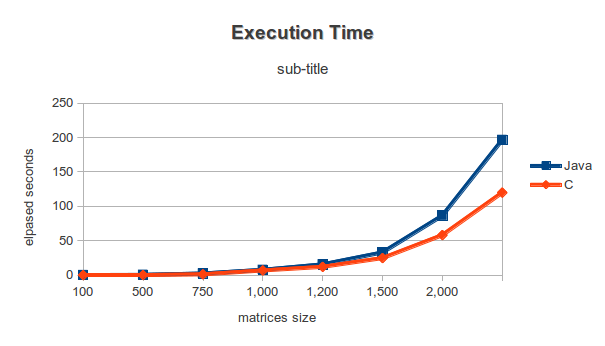
\includegraphics[scale=0.9]{res/pic004}
\caption{Сравнение производительности виртуальной машины Java и нативно исполняемого кода (язык C) на примере задачи перемножения двух матриц.}
\end{figure}

%------------------------------------------------

\section*{Многопоточное программирование}

Параллельное и многопоточное исполнение кода стало трендом последних лет. Во многом это связано с реализацией аппаратной поддержки, получили широкое распространение многоядерные процессоры. Многоядерные процессоры сейчас ставятся не только в сервера и десктопы, но даже в телефоны. Параллельная обработка многих задач (к примеру, обработка изображений) даёт значительно больший выигрыш в производительности, чем банальное увеличение частоты центрального процессора. Это подтверждает рисунок 5 (источник указан под изображением) - начиная с 2005 года частота и потребляемая энергия замерли, но количество транзисторов и производительность продолжили рост. Вместе с тем, это создаёт большое количество проблем, таких как гонки по данным, взаимные блокировки (дедлок и лайвлок), ресурсное голодание. Дополнительно это сопровождается проблемами с аппаратным (когерентность кешей, общая память) и алгоритмическим уклонами (не все алгоритмы хорошо поддаются распараллеливанию, а производительность параллельных проблем лимитируется законом Амдала).

\begin{figure}[h!]
\centering
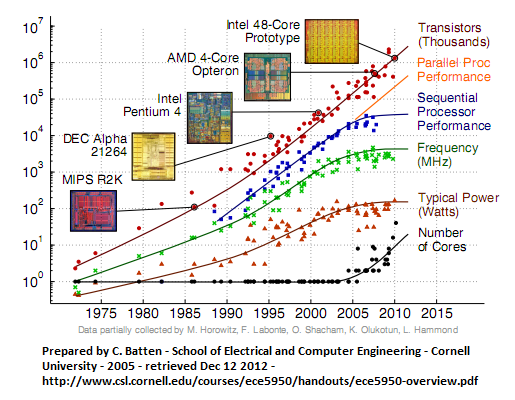
\includegraphics[scale=1]{res/pic005}
\caption{Рост производительности микропроцессоров за счёт использования параллельности.}
\end{figure}

Параллельные программы значительно сложнее поддаются тестированию и отладке, т.к. они лишены такого важного качества как детерминизм. Для демонстрации сложности можно изучить изображение 6. На нём показан граф вызовов, полученный в результате трассировки маленькой программы hello world (его код приводится в листинге 1), использующей стандартную библиотеку MPI (код выполнялся на компиляторе gcc).


\begin{lstlisting}[language=C++, caption={Пример простой многопоточной программы hello world}]
void main (int argc, char *argv[])
{
    int myrank, size;

    MPI_Init(&argc, &argv);
    MPI_Comm_rank(MPI_COMM_WORLD, &myrank);
    MPI_Comm_size(MPI_COMM_WORLD, &size);
    printf("Processor %d of %d: Hello World!\n", myrank, size);
    MPI_Finalize();
}
\end{lstlisting}

Очевидно, что те принципы обеспечения качества (основанные на статическом анализе и ручном тестировании) и верификации кода, которые применялись раньше не подходят для параллельного программирования, и именно это мне кажется наиболее актуальной из современных проблем системного программирования.

\begin{figure}[h!]
\centering
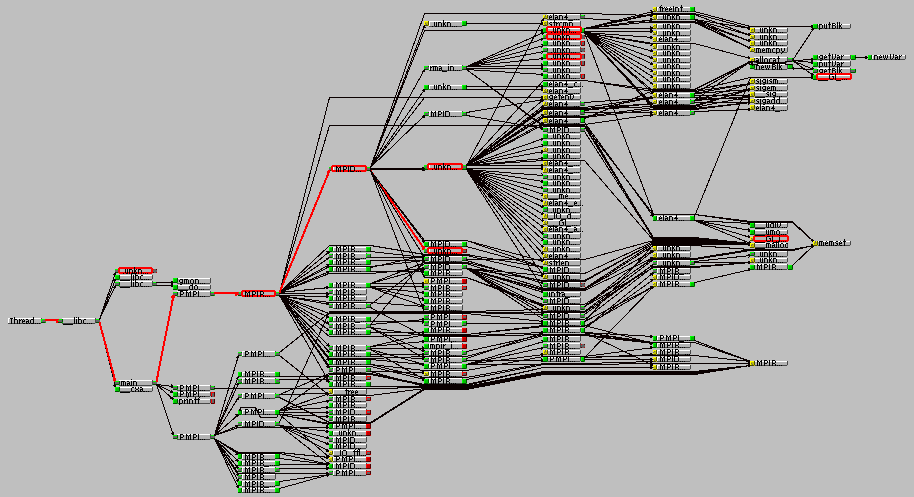
\includegraphics[scale=0.45]{res/pic006}
\caption{Граф вызовов библиотек для простой параллельной программы hello world.}
\end{figure}

%------------------------------------------------

\section*{Заключение}

За последние 10 лет общее количество задач в Системном программировании только увеличивалось. В то же время, для многих задач были сформулированы решения (такие как применение абстракции на всех уровнях), приятые всем сообществом.

В данной работе были упомянуты следующие проблемы:

\begin{enumerate}
\item  увеличение объёмов кода
\item  рост количества "умных устройств" вокруг нас
\item  взаимодействие различных типов устройств
\item  разнообразие платформ
\item  обеспечение безопасности
\item  энергоэффективность
\item  взаимодействие человека и компьютера
\item  виртуализация и построение гипервизоров
\item  виртуальная абстрактная машина для выполнения кода
\item  эффективная и безопасная работа параллельных программ
\end{enumerate}

На мой взгляд самой острой проблемой в данный момент является решение последней проблемы, т.к. параллельное программирование применяется уже достаточно широко, при этом многие разработчики указывают именно эту часть своей работы как основной источник ошибок.

%----------------------------------------------------------------------------------------
%	BIBLIOGRAPHY
%----------------------------------------------------------------------------------------

%\bibliographystyle{unsrt}

%\bibliography{sample}

%\begin{wrapfigure}{l}{0.4\textwidth} % Inline image example
%\begin{center}
%\includegraphics[width=0.38\textwidth]{pic/pic001}
%\end{center}
%\caption{Fish}
%\end{wrapfigure}

%----------------------------------------------------------------------------------------

\end{document}
